\documentclass[../main.tex]{subfiles}
\graphicspath{{\subfix{../img/}}}
\newacronym
  {pren1}                % id
  {PREN 1}                % display name
  {Produktentwicklung 1}  % full acronym name
  
\newacronym
  {pren2}                % id
  {PREN 2}                % display name
  {Produktentwicklung 2}  % full acronym name

\newacronym
  {yaml}
  {YAML}
  {YAML Ain't Markup Language}

\newacronym
  {tof-sensor}
  {ToF-Sensor}
  {Time-of-Flight Sensor}

\newglossaryentry{h-brücke}{
    name={H-Brücke},
    description={
         Eine H-Brücke ist eine Schaltung, die es ermöglicht, einen Elektromotor in beide Richtungen zu betreiben, indem sie den Stromfluss durch den Motor umkehrt. Sie besteht aus vier Schaltern (meistens Transistoren oder MOSFETs), die in einer "H"-Form angeordnet sind. Die Schalter werden so gesteuert, dass der Motor entweder vorwärts, rückwärts oder gestoppt wird.
    }
}


\newglossaryentry{pwm}{
    name={PWM},
    description={
        PWM (Pulsweitenmodulation) ist eine Technik zur Steuerung der Leistung von elektrischen Geräten, wie Motoren oder LEDs, durch das schnelle Ein- und Ausschalten eines Signals. Dabei wird die Dauer, in der das Signal "ein" ist (die Pulsbreite), im Vergleich zur Gesamtdauer eines Zyklus (der Periode) variiert.
    }
}


\newglossaryentry{ir-fototransistor}{
    name={IR-Fototransistor},
    description={
        Ein Fototransistor ist ein Halbleiterbauteil, das Licht in elektrischen Strom umwandelt. Wenn Licht auf den Transistor trifft, verändert sich seine elektrische Leitfähigkeit, was zu einer Stromänderung führt. Ein Infrarot(IR)-Fototransistor reagiert speziell auf Infrarotlicht. 
    }
}


\newglossaryentry{i2c}{
    name={I\textsuperscript{2}C},
    description={
        Eine serielle Kommunikationsschnittstelle, die den Datenaustausch zwischen verschiedenen Komponenten wie Mikrocontrollern, Sensoren und Aktoren über nur zwei Leitungen ermöglicht: \textit{Serial Data Line} für die Datenübertragung und \textit{Serial Clock Line} für die Synchronisation. 
        Die I\textsuperscript{2}C-Schnittstelle unterstützt mehrere Geräte in einem Netzwerk und verwendet Adressen, um einzelne Komponenten anzusprechen.
    }
}


\newglossaryentry{uart}{
    name={UART},
    description={
        Abkürzung für \textit{Universal Asynchronous Receiver Transmitter}. 
        Eine Hardware-Komponente oder ein Kommunikationsprotokoll, das zur seriellen, asynchronen Datenübertragung verwendet wird. 
        UART ermöglicht die Kommunikation zwischen zwei Geräten, indem Daten über eine Sendeleitung (\textit{TX}) und eine Empfangsleitung (\textit{RX}) übertragen werden. Es erfordert keine gemeinsame Taktleitung und verwendet stattdessen Start- und Stoppbits zur Synchronisation. 
    }
}


\newglossaryentry{PLA}{
    name={PLA},
    description={
    Polymilchsäure   (PLA) ist ein biologisch   abbaubarer, thermoplastischer Kunststoff, der aus erneuerbaren Ressourcen wie Maisstärke oder Zuckerrohr hergestellt wird.
    }}

\begin{document}

\newpage
\section{Projektmanagement}

\subsection {Projektorganisation}
PREN ist eine Zusammenarbeit aus drei Studiengängen der Hochschule Luzern - Maschinenbau, Elektrotechnik und Informatik. Das Projektteam ist aus zwei Personen pro Disziplin zusammengesetzt. Die Organisationsform für PREN ist frei wählbar. Das Team entschied sich, keinen festen Projektleiter zu benennen. Stattdessen wurden Projektmanagement, Steuerung und Kontrolle im wöchentlichen Austausch gemeinsam übernommen und die Aufgaben auf alle Mitglieder verteilt.

\subsection{Projektziele des Teams}
Das Team formulierte zu Beginn des Projekts klare Ziele. Folgende projektumfassende Ziele wurden gewählt:
\begin{itemize}
\item \textbf{Einfach:} Das Team möchte ein möglichst einfaches Lösungskonzept entwickeln, das alle Anforderungen der Aufgabenstellung erfüllt.
\item \textbf{Zuverlässig:} Das Fahrzeug soll die Aufgabe aus der Aufgabenstellung zuverlässig lösen (>95\%) und dies am Wettbewerb vorführen.
\end{itemize}

Diese Ziele bieten die Grundlage für das Fahrzeug inklusive Software.
Die Positionierung im Wettbewerb in \acrshort{pren2} ist durch die Zielsetzung klar sekundär. Durch das zuverlässige Lösen der Aufgabe, \textcolor{red}{wird eine Platzierung sichergestellt. Was ist mit Platzierung gemeint?}

\subsection{Resultate und Umfang}
Für PREN1 wurden in der Aufgabenstellung (siehe Anhang \ref{aufgabenstellung}) drei Meilensteine und deren Resultate definiert. Weitere Meilensteine sind aus den Semesterterminen abgeleitet.
\begin{table}[H]
\centering
\begin{tabular}{|l|l|p{10cm}|}
\hline
\textbf{Meilenstein} & \textbf{Abgabe} & \textbf{Resultate} \\ \hline
 1        & 04.10.2024      & Projektplanung, Skizzierung / Modell der Aufgabenstellung, Technologierecherche, Anforderungsliste \\ \hline
 2        & 01.11.2024      & Evaluation der Lösungsprinzipien, Auswahl der optimalen Lösungskombination(en) \\ \hline
 3        & 06.12.2024      & Gesamtkonzept inkl. „Simulator Wegplanung“, Dokumentation zu 80\% fertiggestellt \\ \hline
 4        & 10.01.2025      &  Schlussbericht Projektdokumentation Lösungskonzept, Präsentation Lösungskonzept\\ \hline 
 
\end{tabular}
\caption{Meilensteine und Resultate}
\label{tab:meilensteine}
\end{table}


\subsection{Risikomanagement} \label{risikomatrix}

Alle bekannten Risiken in Bezug zum Projekt sind in Tabelle \ref{tab:risikotabelle} aufgelistet. Diese Risiken werden kontinuierlich erweitert und möglichst minimiert. Dies kann beispielsweise anhand von Prototypen, geplanten Backup-Lösungen oder vertieften Recherchen erfolgen.

Dabei hat jedes Risiko folgende Attribute:
\begin{itemize}
    \item \textbf{Titel + Beschreibung}: Beschreibung des Risikos
    \item \textbf{Verantwortlich} Welche Gruppe dafür verantwortlich ist (INF=Informatik, MT=Maschinentechnik, ET=Elektrotechnik).
    \item \textbf{Kategorie}: In welcher Kategorie sich das Risiko befindet.
    \item \textbf{Ursachen}: Was passieren muss, damit das Risiko eintreffen kann.
    \item \textbf{Bewertung des Risikos}: Eintrittswahrscheinlichkeit, Auswirkung und Risiko Bewertung ohne Massnahmen
    \item \textbf{Massnahmen zur Risikominimierung}: Massnahmen um die Eintrittswahrscheinlichkeit oder Auswirkung zu minimieren.
    \item \textbf{Korrekturmassnahmen}: Was gemacht werden soll, wenn das Risiko trotzdem Eintrifft
    \item \textbf{Erfolgsfaktoren}: Beschreibt das Verhalten bei erfolgreicher Risikomitigation
    \item \textbf{Erneute Bewertung des Risikos}: Eintrittswahrscheinlichkeit, Auswirkung und Risiko Bewertung mit den definierten Massnahmen
\end{itemize}

Aus Darstellungsgründen wurden die Attribute der Risikos in zwei Reihen aufgeteilt. In der ersten Reihe werden die Risikos und ihre Auswirkungen genannt und bewertet, sowie die Verantwortlichkeit definiert. In der zweiten Reihe werden die Massnahmen zur Risikominderung, die Korrekturmassnahmen und die Erfolgsfaktoren genannt, weiter wird dazu nochmal eine Bewertung gemacht.

\begin{landscape}
\newpage
\scriptsize

\textbf{Legende:}
\hspace{1cm}
\textbf{VW:} Verantwortlich
\hspace{1cm}
\textbf{EW:} Eintrittswahrscheinlichkeit (1-5)
\hspace{1cm}
\textbf{AW:} Auswirkung (1-5)
\hspace{1cm}
\textbf{BW:} Bewertung (EW * AW)
\\
\vspace{1mm} \hspace{21.5mm}
\textbf{EWM:} EW mit Massnahmen (1-5)
\hspace{1cm}
\textbf{AWM:} AW mit Massnahmen  (1-5)
\hspace{1cm}
\textbf{BWM:} BW mit Massnahmen (EW * AW)


\renewcommand{\arraystretch}{1.5} % Adjust row height for readability
\setlength{\arrayrulewidth}{0.6pt}
\begin{longtable}
{|c|p{4.5cm}|p{5cm}|c|c|p{4.5cm}|c|c|c|}
\hline
\rowcolor{white}
& \textbf{Titel} & \textbf{Beschreibung} & & & \textbf{Ursachen} & \textbf{EW} & \textbf{AW} & \textbf{BW} \\ 
\cline{2-3} \cline{6-9}
\rowcolor{white}
\multirow{-2}{*}{\textbf{ID}}
& \textbf{Massnahmen Risikominderung} & \textbf{Korrekturmassnahmen} & \multirow{-2}{*}{\textbf{VW}} & \multirow{-2}{*}{\textbf{Kategorie}} & \textbf{Erfolgsfaktoren} & \textbf{EWM} & \textbf{AWM} & \textbf{BWM} \\ \hline
\endhead

\rowcolor[HTML]{F5F5F5} & \textbf{Grip-Verlust normale Räder} & Das Fahrzeug schleift über den Boden & MT & Mechanisch & Fahrzeug verliert Grip & 3 & 3 & \cellcolor[HTML]{FFFF66}9
\\* \cline{2-3} \cline{6-9}
\rowcolor[HTML]{F5F5F5} \multirow{-2}{*}{\hypertarget{R1}{R1}} & Auf Mensaboden testen & Andere Räder/Geschwindigkeit anpassen & & & Fahrzeug hat Grip & 2 & 2 & \cellcolor[HTML]{CCFF33}4 \\ \hline

\rowcolor{white} & \textbf{Liniensensor falsche Daten} & Der Liniensensor erkennt die Fugen als Führungslinie & ET+INF & Elektrisch & Fahrzeug folgt der Fuge & 4 & 4 & \cellcolor[HTML]{FFC000}16
\\* \cline{2-3} \cline{6-9}
\rowcolor{white} \multirow{-2}{*}{\hypertarget{R2}{R2}} & Kalibrierung des Sensors, Abgleich mit Kamera & Not-Aus verwenden & & & Fahrzeug folgt Führungslinie & 2 & 5 & \cellcolor[HTML]{FFC000}10 \\ \hline

\rowcolor[HTML]{F5F5F5} & \textbf{Motorenposition ungenau} & Für Rückstellen des Hindernis ungenau Positionswerte & ET & Elektrisch & Hindernis nicht innerhalb 2 cm & 3 & 3 & \cellcolor[HTML]{FFFF66}9 \\* \cline{2-3} \cline{6-9}
\rowcolor[HTML]{F5F5F5} \multirow{-2}{*}{\hypertarget{R3}{R3}} & Langsame Fahrt bei Positionierung & Hallsensor, Drehgeber, Schrittmotor & & & Hindernis innerhalb der 2 cm Toleranz & 2 & 2 & \cellcolor[HTML]{CCFF33}4 \\ \hline

\rowcolor{white} & \textbf{Distanzmessung fehlerhafte Daten} & Für die Erkennung der Distanz, des Hindernis, könnten falsche Messwerte eine ungewollte Aktion ausführen & ET & Elektrisch & Fahrzeug führt Hindernisbewältigung aus ohne ein Hindernis & 2 & 2 & \cellcolor[HTML]{CCFF33}4 \\* \cline{2-3} \cline{6-9}
\rowcolor{white} \multirow{-2}{*}{\hypertarget{R4}{R4}} & Distanzwert muss längere Zeit konstant bleiben & Zweiter Sensor zum Vergleich verbauen & & & Fahrzeug führt Hindernisbewältigung nur bei einem Hindernis aus & 1 & 2 & \cellcolor[HTML]{00CC00}2 \\ \hline

\rowcolor[HTML]{F5F5F5} & \textbf{Datenverlust} & Verlust von Projektdaten/Forschungsergebnissen & INF & Projekt & Server offline & 2 & 5 & \cellcolor[HTML]{FFC000}10 \\* \cline{2-3} \cline{6-9}
\rowcolor[HTML]{F5F5F5} \multirow{-2}{*}{\hypertarget{R5}{R5}} & Regelmässige Backups erstellen & Daten aus Backups wiederherstellen & & & Daten sind zugänglich und schnell wiederherstellbar & 2 & 2 & \cellcolor[HTML]{CCFF33}4 \\ \hline

\rowcolor{white} & \textbf{Lieferschwierigkeiten} & Teile, die bestellt werden haben Lieferverzögerung & ET+MT &  Market & Längere Lieferzeiten/Keine Lieferzeiten angegeben & 3 & 4 & \cellcolor[HTML]{FFC000}12 \\* \cline{2-3} \cline{6-9}
\rowcolor{white} \multirow{-2}{*}{\hypertarget{R6}{R6}} & Frühzeitig Bestellen, alternative Teile/Quellen suchen & bei alternativen Quellen bestellen & & & Teile können zeitnah verwendet verbaut werden & 3 & 3 & \cellcolor[HTML]{FFFF66}9 \\ \hline

\rowcolor[HTML]{F5F5F5} & \textbf{Software-Absturz} & Software crasht während Einsatz & INF & Software & Prozess wird unerwartet beendet & 2 & 5 & \cellcolor[HTML]{FFC000}10 \\* \cline{2-3} \cline{6-9}
\rowcolor[HTML]{F5F5F5} \multirow{-2}{*}{\hypertarget{R7}{R7}} & Gutes Testen des Codes und Failsafe einbauen & Not-Aus verwenden & & & Fahrzeug kann nach Absturz von alleine wieder starten & 1 & 5 & \cellcolor[HTML]{FFFF66}5 \\
\hline
\rowcolor{white} & \textbf{Verlust Sensorkommunikation} & Die Kommunikation zwischen Sensorik und Software ist gestört & ET+INF & Software & Fehlerhafte Daten oder fehlende Daten & 2 & 5 & \cellcolor[HTML]{FFC000}10 \\* \cline{2-3} \cline{6-9}
\rowcolor{white} \multirow{-2}{*}{\hypertarget{R8}{R8}} & Sicheres verbauen und Testen der Sensoren & Neueinstellung/Kalibrierung durchführen & & & Fahrzeug kann trotz fehlerhafter Sensordaten Aufgabe erfüllen & 2 & 3 & \cellcolor[HTML]{CCFF33}6 \\ \hline

\pagebreak

\rowcolor[HTML]{F5F5F5} & \textbf{Software zu anspruchsvoll für Computer} & Die Leistung des Computers reicht nicht aus & INF & Software & Software-Lags, langsame Reaktionszeit & 3 & 4 & \cellcolor[HTML]{FFC000}12 \\* \cline{2-3} \cline{6-9}
\rowcolor[HTML]{F5F5F5} \multirow{-2}{*}{\hypertarget{R9}{R9}} & Software optimiert bauen & Langsamer fortsetzen & & & Fahrzeug kann trotz langsamer Laufzeit Aufgabe lösen & 3 & 3 & \cellcolor[HTML]{CCFF33}9 \\ \hline
\rowcolor{white} & \textbf{Pylone wird überfahren} & Eine Pylone wird nicht erkannt & ET+INF & Elektrisch & Pylone wird nicht erkannt & 3 & 5 & \cellcolor[HTML]{FFC000}15 \\* \cline{2-3} \cline{6-9}
\rowcolor{white} \multirow{-2}{*}{\hypertarget{R10}{R10}} & Frühes Training und Testing & Not-Aus verwenden & & & Das Fahrzeug erkennt Pylonen & 1 & 5 & \cellcolor[HTML]{FFFF66}5 \\ \hline

\rowcolor[HTML]{F5F5F5} & \textbf{Unscharfe Bilder während Fahrt} & Kamera liefert unscharfe Bilder & MT+INF & Software & Objekterkennung fehlerhaft & 4 & 4 & \cellcolor[HTML]{FFC000}16 \\* \cline{2-3} \cline{6-9}
\rowcolor[HTML]{F5F5F5} \multirow{-2}{*}{\hypertarget{R11}{R11}} & Bildaufnahme nur bei stehendem Fahrzeug & Fahrzeug stehen lassen & & & Das Fahrzeug erkennt Objekte korrekt & 2 & 4 & \cellcolor[HTML]{FFFF66}8 \\ \hline

\rowcolor{white} & \textbf{Fokus der Kamera} & Fokus umfasst nicht benötigten Bereich & ET+INF & Elektrisch & Objekte werden nicht korrekt erkannt & 3 & 3 & \cellcolor[HTML]{FFFF66}9 \\* \cline{2-3} \cline{6-9}
\rowcolor{white} \multirow{-2}{*}{\hypertarget{R12}{R12}} & Fokus-Range prüfen & Software anpassen & & & Fahrzeug erkennt Objekte & 2 & 2 & \cellcolor[HTML]{CCFF33}4 \\ \hline

\rowcolor[HTML]{F5F5F5} & \textbf{Grip-Verlust Omni/Mecanum} & Fahrzeug verliert Grip bei Fugen & MT & Mechanisch & Fahrzeug verliert Grip & 4 & 4 & \cellcolor[HTML]{FFC000}16 \\* \cline{2-3} \cline{6-9}
\rowcolor[HTML]{F5F5F5} \multirow{-2}{*}{\hypertarget{R13}{R13}} & Testen der Räder & Mit Sensoren Position ausgleichen & & & Fahrzeug ist an gewünschter Position & 3 & 3 &\cellcolor[HTML]{FFFF66} 9 \\ \hline

\rowcolor{white} & \textbf{Anzahl GPIO} & Steuerung hat begrenzte Pins & ET & Elektrisch & Sensorinformationen nicht lesbar & 3 & 5 & \cellcolor[HTML]{FFC000}15 \\* \cline{2-3} \cline{6-9}
\rowcolor{white} \multirow{-2}{*}{\hypertarget{R14}{R14}} & Erweiterung mit Multiplexern & Alternative Schaltungen & & & Sensorinformationen verfügbar & 3 & 4 & \cellcolor[HTML]{FFC000}12 \\ \hline

\rowcolor[HTML]{F5F5F5} & \textbf{Verschiebung bei Drehung} & Keine genaue Drehung möglich & MT & Mechanisch & Fahrzeug schiebt seitlich & 3 & 5 & \cellcolor[HTML]{FFC000}15 \\* \cline{2-3} \cline{6-9}
\rowcolor[HTML]{F5F5F5} \multirow{-2}{*}{\hypertarget{R15}{R15}} & Testen & Zusatzfunktion abdocken & & & Fahrzeug dreht fix & 2 & 2 & \cellcolor[HTML]{CCFF33}4 \\ \hline

\rowcolor{white} & \textbf{Blendende Beleuchtung} & Licht stört Kamera & ET & Elektrisch & Kamera sieht Blendung statt Objekt & 4 & 4 & \cellcolor[HTML]{FFC000}16 \\* \cline{2-3} \cline{6-9}
\rowcolor{white} \multirow{-2}{*}{\hypertarget{R16}{R16}} & LEDs vermeiden & Kameraeinstellung bei wenig Licht & & & Kamera erkennt Objekt trotz Blendung & 2 & 3 & \cellcolor[HTML]{CCFF33}4 \\ \hline

\rowcolor{white} & \textbf{Reflexion bei Distanzmessung} & Messfehler, wenn Objekte in der Nähe der Linie sind, aber nicht relevant sind für die Messung& ET & Elektrisch & Kein Objekt auf Fahrweg, detektiert Objekt& 3 & 3 & \cellcolor[HTML]{FFC000}9 \\* \cline{2-3} \cline{6-9}
\rowcolor{white} \multirow{-2}{*}{\hypertarget{R17}{R17}} & Distanz beschränken, für die Sensorwerte akzeptiert werden. Objekterkennung für kurze Zeit nach Drehung ignorieren
 & Kameraeinstellung bei wenig Licht & & & Erkennt das Hinderniss in der richtigen Distanz& 1 & 3 & \cellcolor[HTML]{CCFF33}3 \\ \hline

\caption{Risikotabelle}
\label{tab:risikotabelle}

\end{longtable}
\normalsize    
\end{landscape}

\newpage

\begin{figure}[H]
    \centering
    \begin{subfigure}[t]{0.5\textwidth}
        \centering
        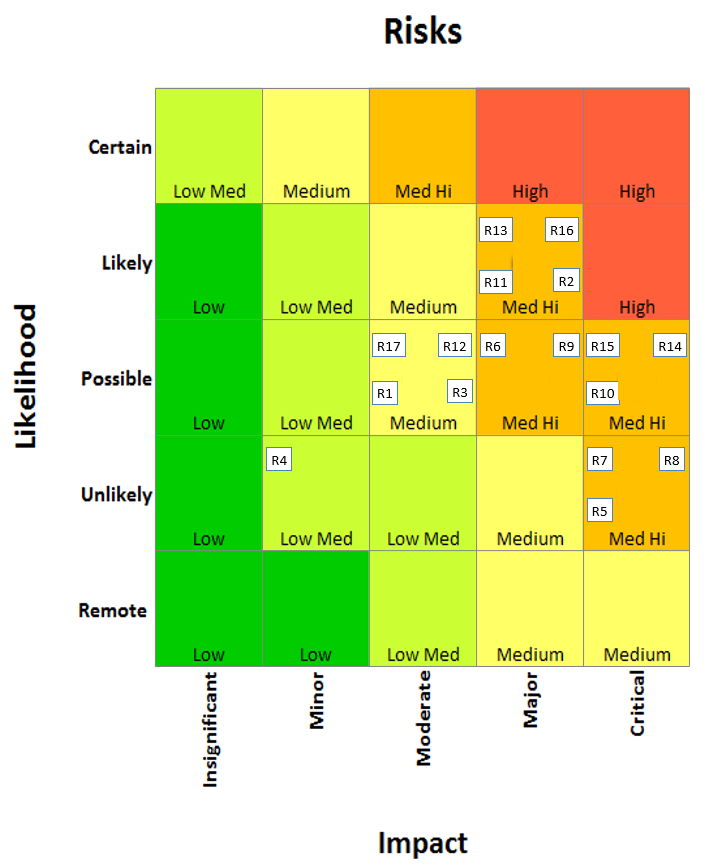
\includegraphics[width=8cm]{img/Risikomatrix/Risks_before_measures_v2_pren1.png}
        \caption{Risikomatrix vor Massnahmen}
    \end{subfigure}%
    ~ 
    \begin{subfigure}[t]{0.5\textwidth}
    \centering
       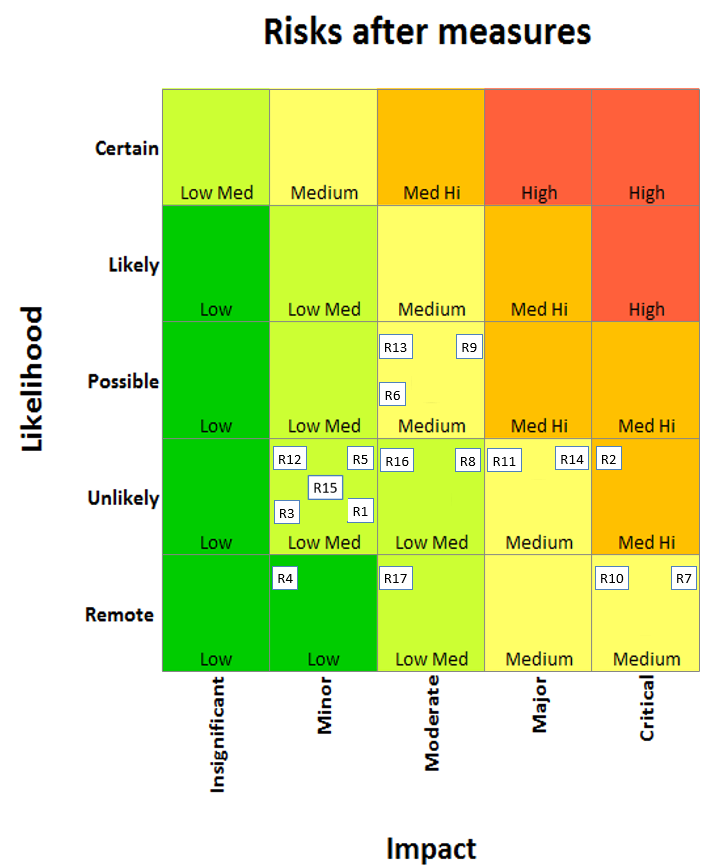
\includegraphics[width=8cm]{img/Risikomatrix/Risks_after_measures_v2_pren1.png}
       \caption{Risikomatrix nach Massnahmen}
    \end{subfigure}
    \label{fig:risikomatrix}
    \caption{Vergleich Risikomatrix vor und nach risikomindernden Massnahmen.}
\end{figure}

In der Abbildung \ref{fig:risikomatrix} ist ersichtlich, dass mit den risikomindernden Massnahmen eine klare Reduktion der Eintrittswahrscheinlichkeit sowie der Schwere der Konsequenzen erreicht wird. Gewisse Risiken müssen dennoch in Kauf genommen werden.

\subsection{Projektplan}
Für die Projektplanung wird eine Excel-Vorlage verwendet. Die geplanten und benötigten Tage, sowie Verzögerungen und früherer Abschluss werden im Projektplan dargestellt. Meilensteine sowie die dazugehörigen Aufgaben sind hier festgehalten und werden regelmässig aktualisiert. Anhand dieses Plans wird das Projekt-Controlling durchgeführt.
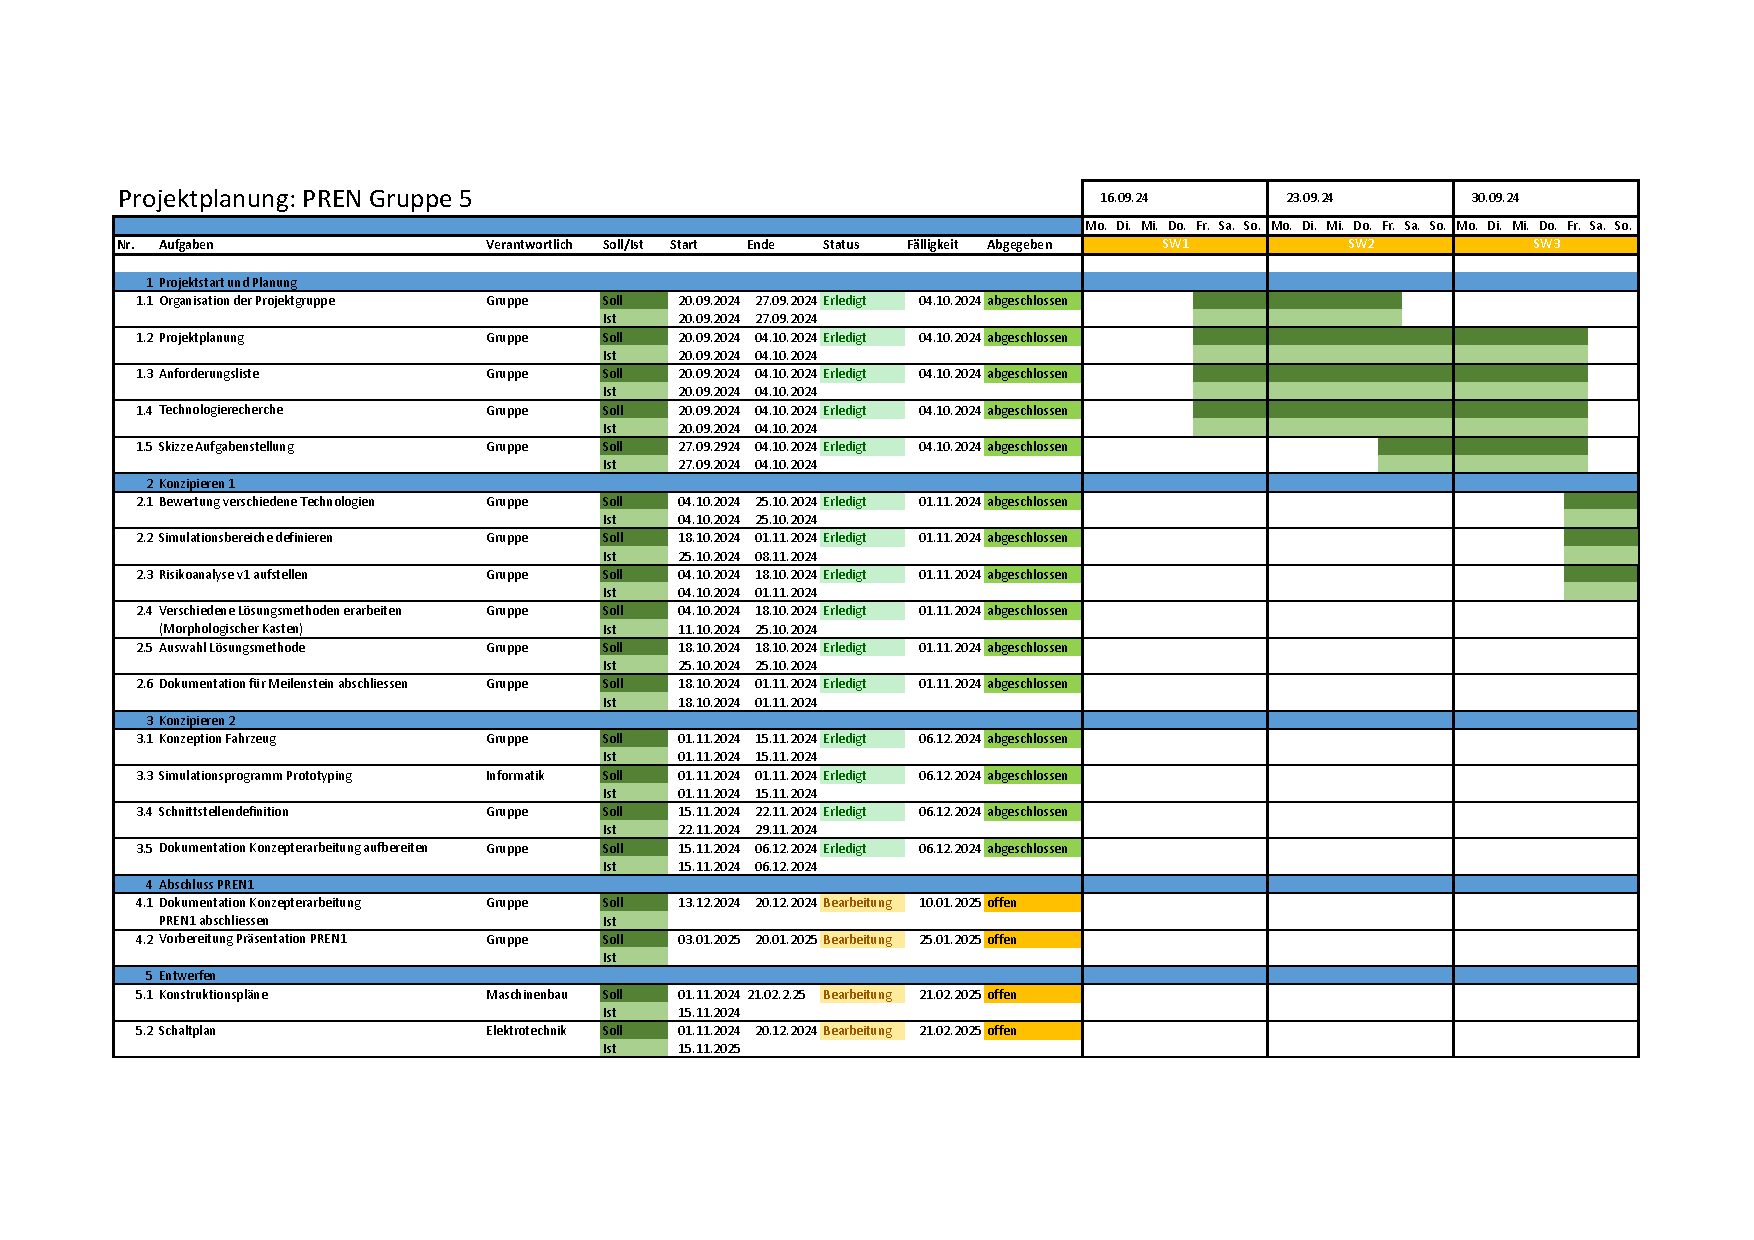
\includepdf[
  landscape=true,
  pages={1-},
  scale=1,
  pagecommand={\pagestyle{fancy}}
]{assets/Projektplan_v6.pdf}

\subsection{Werkzeuge}

Verschiedene Werkzeuge unterstützen das Projekt in unterschiedlichen Bereichen. Diese werden in der Tabelle \ref{tab:werkzeugtabelle} festgehalten.

\begin{table}[H]
\centering
\begin{tabular}{|l|l|}
\hline
\textbf{Werkzeug} & \textbf{Gebraucht für} \\ \hline
Visual Studio Code & Simulator-/Software-Entwicklung \\ \hline
Unreal Engine 5 & Erstellung virtueller Klon \\ \hline
Blender & Konvertierung 3D Modelle und Texturierung \\ \hline
Overleaf & Erstellung Dokumentation \\ \hline
Github & Host für Code Repositories und Backup Dokumentation \\ \hline
Altium Designer & Elektronik Schema + PCB-Layouts \\ \hline
NX Siemens & Zeichnen von 3D Modellen \\ \hline
Concept & Zeichnen von Skizzen \\ \hline
Draw.io & Diagramme erstellen \\ \hline
Roboflow & Bilder für Objekterkennung annotieren \\ \hline
Microsoft Excel & Projektplan und Risikomatrix \\ \hline
Microsoft Teams & Dateiablage und Kommunikationshub \\ \hline
Chat-GPT & Proof-Reading \\ \hline
KissSoft & Auslegen der Zahnräder \\ \hline
 
\end{tabular}
\caption{Tabelle der verwendeten Werkzeuge für PREN}
\label{tab:werkzeugtabelle}
\end{table}


\subsection{Produktkostenkontrolle}
Das Projekt hat einen fixen Budgetrahmen von total CHF 500.--, wobei maximal CHF 200.-- in PREN1 ausgegeben werden dürfen. Eine Kostenkontrolle dokumentiert die getätigten Ausgaben und die geplanten Kosten für PREN2.
\begin{table}[H]
\begin{tabular}{|p{6cm}|p{2.5cm}|p{2cm}|p{2.5cm}|}
\hline
\textbf{Was} & \textbf{Preis} & \textbf{Gekauft} & \textbf{Wo} \\ \hline
Raspberry Pi Module 3 Kamera & CHF 37.30 & 31.10.2024 & Digitec \\ \hline
Raspberry Pi 5 8GB & CHF 77.90 & 09.11.2024 & Digitec \\ \hline
Kamera-Kabel & CHF 5.70 & 11.11.2024 & Digitec \\ \hline
H Brücke A4950 & CHF 3.06 & 22.11.2024 & Mouser \\ \hline
DC-Motor mit Encoder & CHF 32.10 & 22.11.2024 & Mouser \\ \hline
IR-LED & CHF 3.30 & 22.11.2024 & Mouser \\ \hline
Phototransistor & CHF 4.30 & 22.11.2024 & Distrelec \\ \hline
\hline
\textbf{Total} & \textbf{CHF 163.66} & & \\ \hline
\end{tabular}
\caption{Tabelle aller Ausgaben in PREN1}
\label{tab:ausgaben_pren1}
\end{table}

\begin{table}[H]
\begin{tabular}{|p{6cm}|p{2.5cm}|p{2cm}|p{2.5cm}|}
\hline
\textbf{Was} & \textbf{Preis} & \textbf{Gekauft} & \textbf{Wo} \\ \hline
Total Ausgaben PREN1 & CHF 163.66.-- &  &  \\ \hline
Elektronische Bauteile und Baugruppen & CHF 100.-- &  &  \\ \hline
PCB des Adapterboards & CHF 80.-- &  &  \\ \hline
Gehäuse, Räder und Mechanismus & CHF 100.-- &  &  \\ \hline
\hline
\textbf{Total} & \textbf{CHF 443.66} & & \\ \hline
\end{tabular}
\caption{Tabelle der geplanten Ausgaben bis Ende PREN2}
\label{tab:ausgaben_pren2}
\end{table}

\end{document}